\section{Testy}
  \label{testy}
  Technologie internetowe rozwijają się bardzo szybko, a co za tym idzie, wymagania klientów również. Wiele firm kładzie duży nacisk na testowanie swoich aplikacji.

  Programiści często wychodzą z założenia, że ,,najpierw kod, później testy". Ma to oczywiście swoje wady i zalety. Zaletą niewątpliwie jest czas realizacji. W pierwszej kolejności dostarcza się funkcjonalności i nie zastanawia się nad tym jak napisać do nich testy. Pod koniec procesu produkcji tworzy się kilka testów sprawdzających zachowanie aplikacji. Doprowadza to do tego, że cały kod aplikacji pokryty jest testami w bardzo niewielkim stopniu. W każdej chwili może zajść sytuacja, w której aplikacja przestanie działać zgodnie z założeniami. Niestety w takim przypadku tracimy cenne godziny na szukanie błędów i ich eliminację.

  Podczas tworzenia aplikacji Meetspace przyjęliśmy zupełnie inne podejście - „najpierw testy, później kod". Czas pisania aplikacji znacznie się wydłużył. Osiągnęliśmy jednak bardzo dobre pokrycie kodu testami. \\ \\
    (dać tu wykres STATS - metryki i krótko omówić go, gdyż jest tam duży skok) \\ \\
  Dzięki napisanym testom oszczędziliśmy sporo godzin przy diagnozowaniu błędów aplikacji. Kolejną zaletą obranego podejścia jest to, że napisany w ten sposób przez nas kod robi dokładnie to czego oczekujemy. Każdy test spełniany jest w najprostszy możliwy sposób. Na jedną metodę przypada kilka lub nawet kilkanaście testów. Jeżeli któryś z nich się nie spełni, wiadomo od razu gdzie szukać przyczyny.

  \subsection{Techniki tworzenia oprogramowania}
    Techniki tworzenia oprogramowania są niezwykle ważne w całym procesie powstawania kodu. Pomagają efektywnie zarządzać zasobami zespołu, czasem, zadaniami i celami, które stoją przed \emph{team'em}.

    Poniżej krótko objaniśmy te techniki, z których korzystaliśmy.
    \index{TDD}
    \begin{itemize}
      \item Test Driven Development\cite{tdd} \\
        Technika tworzenia oprogramowania, sterowana przez testy. Polega na wielokrotnym powtarzaniu 3 kroków do momentu ukończenia funkcjonalności:
        \begin{enumerate}
          \item Napisanie możliwie najprostszego testu jednostkowego, który ma sprawdzać kod pisany w kroku 2.
          \item Implementacja kodu. Kod powinien być napisany w taki sposób, aby spełnić założenia testu, nic ponad to. Test powinien zakończyć się sukcesem i nie naruszać pozostałych testów
          \item Refaktoryzacja. Doprowadzenie kodu do stanu, w którym spełnia przyjęte normy i standardy prostego oraz czytelnego kodu\cite{scs}.
        \end{enumerate}

        Postępowanie według tego schematu, zmusza programistę do wcześniejszego przemyślenia funkcjonalności, którą ma napisać.

        Wady:
        \begin{itemize}
          \item Wydłuża się czas pisania aplikacji, zwłaszcza w początkowej fazie wdrażania tej techniki. Jednak wraz z ilością napisanych testów jednostkowych, rośnie wydajność ich pisania.
          \item Wraz z rozwojem aplikacji rośnie również ilość testów. Dopóki funkcjonalności są dopisywane, problem nie istnieje. Zmiana funkcjonalności narzuca zmiany po stronie istniejących do niej testów.
        \end{itemize}

        Zalety:
        \begin{itemize}
          \item Główną zaletą tej metodologii jest szybkość diagnozowania błędów. Dzięki temu oszczędzamy mnóstwo czasu. Bez testów musielibyśmy poświęcić go na dogłębną analizę kodu.
          \item Jeżeli testy są pisane w odpowiedni sposób, mogą stanowić bardzo dobrą dokumentację. Wystarczy zajrzeć do testu i widać czego programista oczekiwał od konkretnej metody.
          \item Bardziej przemyślany kod. W pierwszej kolejności musimy się zastanowić co tak naprawdę ma zawierać dana funkcjonalność, żeby móc od niej to wyegzekwować.
        \end{itemize}

        \begin{figure}
          \centering
          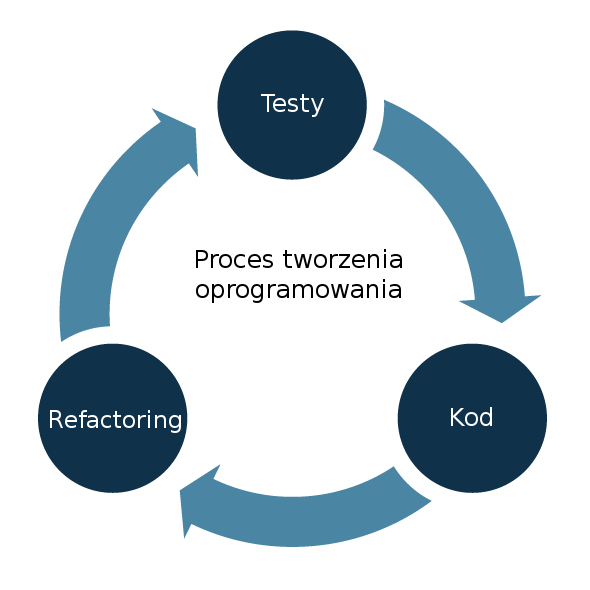
\includegraphics[scale=0.47]{images/test_cycle.png}
          \caption{Schemat postępowania w TDD}
        \end{figure}

      \newpage
      \index{BDD}
      \item Behaviour Driven Development \\
        Technika stworzona przez Dana Northa w 2003 roku. Sam autor powiedział:
        \begin{quote}
          \emph{„Behaviour-driven Development polega na tworzeniu oprogramowania przez opisywanie jego zachowania, z perspektywy jego udziałowców.”}
        \end{quote}

        Dzięki takiej metodyce testowania programiści wychodzą naprzeciw klientowi, starają się go zrozumieć i spełnić jego wymagania.

        Oczekiwania klienta są zapisywane w postaci krótkich historyjek, scenariuszy.
        Podczas ich tworzenia korzysta się z trzech głównych słów kluczowych:
          \begin{itemize}
            \item Podane (\emph{Given}) - opisuje stan początkowy aplikacji
            \item Kiedy (\emph{When}) - wszystkie kroki jakie klient/użytkownik musi wykonać aby osiągnąć funkcjonalność
            \item Wtedy (\emph{Then}) - stan końcowy aplikacji, czyli oczekiwany efekt po przejściu przez wcześniejsze kroki
          \end{itemize}

        \emph{Test driven development} to testowanie na poziomie kodu, \emph{behaviour driven development} to testowanie na poziomie aplikacji. Dlatego jeśli korzysta się z obu technik, zaczyna się od BDD, schodząc coraz ,,niżej'', aż do TDD. Wtedy mamy pewność, że konkretna funkcjonalność jest należycie przetestowana i spełnia oczekiwania oraz wymogi klienta.
    \end{itemize}

  \subsection{Testy integracyjne}
    \index{Cucumber}
    Najważniejszą funkcjonalnością w naszej aplikacji jest kreowanie nowego wydarzenia. Poniżej przedstawimy proces tworzenia testu integracyjnego.

    Pierwszym krokiem jest opisanie w kilku słowach funkcjonalności.
\begin{code}
	\lstinputlisting[linerange={0-4}]{../meetspace/features/events.feature}
\end{code}\\

Następnie tworzymy scenariusz, w którym krok po kroku będziemy wykonywać czynności aż otrzymamy efekt końcowy. W tym przypadku będzie to wyświetlenie nowo dodanego wydarzenia.

Słowem kluczowym ,,Scenario'' nadajemy tytuł nowego scenariusza. Jest to o tyle pomocne, że w momencie uruchomienia testów, widać który scenariusz jest w tej chwili testowany.

\begin{code}
	\lstinputlisting[linerange={10-10}, firstnumber=5]{../meetspace/features/events.feature}
\end{code}\\

Słowem ,,Given'' definiujemy stan początkowy aplikacji, czyli miejsce, w którym będziemy zaczynać wykonywanie konkretnych czynności. W tym przypadku jest to strona główna oraz proces logowania. Zalogowanie się do aplikacji jest istotnym elementem, ponieważ, bez tego nie będziemy w stanie dodać żadnego nowego wydarzenia.

\begin{code}
	\lstinputlisting[linerange={7-8}, firstnumber=6]{../meetspace/features/events.feature}
\end{code}\\

\clearpage

Następnie użytkownik aby utworzyć wydarzenie musi kliknąć przycisk ,,Utwórz wydarzenie'', oraz wypełnić formularz odpowiednimi danymi: nazwa, data, data zakończenia, czas rozpoczęcia, plan i logo.

\begin{code}
	\lstinputlisting[linerange={11-20}, firstnumber=8]{../meetspace/features/events.feature}
\end{code}\\

Po słowie ,,Then'' definiujemy nasze oczekiwania. W tym przypadku chcemy zobaczyć nowo dodane wydarzenie wraz z jego wszystkimi właściwościami. Słowa ,,And'' używamy jeśli chcemy rozwinąć listę wykonywanych kroków lub listę oczekiwań.

\begin{code}
	\lstinputlisting[linerange={21-26}, firstnumber=18]{../meetspace/features/events.feature}
\end{code}\\

W ten sposób mamy opisaną, za pomocą testu integracyjnego, całą ścieżkę, którą musi przejść użytkownik, aby stworzyć nowe wydarzenie.

W przypadku gdy chcemy przetestować edytowanie istniejącego już wpisu, nie musimy przechodzić procesu tworzenia od początku. Wystarczy, że na wstępie stworzymy już gotowe wydarzenie, które w następnych krokach będzie modyfikowane.

\begin{code}
	\lstinputlisting[linerange={28-31}, firstnumber=1]{../meetspace/features/events.feature}
\end{code}\\

W tej chwili w bazie testowej mamy zapisany jeden rekord. Dane z jakimi tworzone jest wydarzenie nie mają w tym momencie najmniejszego znaczenia, nie to jest tutaj testowane. Równie dobrze można by wpisać dowolny ciąg znaków, ale kierujemy się dobrą praktyką programistyczną i staramy się pisać zrozumiały kod.

Aby móc edytować jakikolwiek wpis, musimy wejść na jego stronę i kliknąć odpowiedni przycisk, bądź link, żeby przejść do strony z formularzem.

\begin{code}
	\lstinputlisting[linerange={32-33}, firstnumber=3]{../meetspace/features/events.feature}
\end{code}\\

Zmieniamy wpisane wartości na ,,Party'' oraz ,,15:00 Start'' oraz ustawiamy nowe logo.

\begin{code}
	\lstinputlisting[linerange={34-37}, firstnumber=5]{../meetspace/features/events.feature}
\end{code}\\

I na koniec oczekujemy, że wprowadzone przed chwilą zmiany zobaczymy na stronie wydarzenia.

\begin{code}
	\lstinputlisting[linerange={38-39}, firstnumber=9]{../meetspace/features/events.feature}
\end{code}\\

Można łatwo zauważyć, że część kroków powtarza się w pierwszym jak i w drugim scenariuszu. Jest to nic innego jak zastosowanie metody DRY\footnote{Don't repeat yourself - Nie powtarzaj się}. Dzięki temu nowe testy powstają coraz szybciej i sprawniej.

W całym projekcie testów integracyjnych jest znacznie więcej. Oprócz wyżej pokazanego przykładu, testujemy również logowanie do aplikacji poprzez portal Facebook, wyszukiwanie wydarzeń, czy zapisywanie się na newsletter.

Poniżej przedstawiony jest rezultat wszystkich testów integracyjnych. W sumie 12 scenariuszy i 78 kroków, wszystkie spełnione pomyślnie.

\begin{figure}[h]
  \centering
  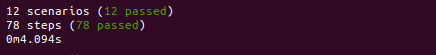
\includegraphics[scale=0.8]{images/bdd_result.png}
  \caption{Wyniki końcowe testów integracyjnych.}
\end{figure}

\newpage

  \subsection{Testy jednostkowe}
    \index{RSpec}
    Testy jednostkowe weryfikują działanie pojedynczych elementów(jednostek) programu, poszczególnych metod czy relacji między obiektami. Taki test wykonuje dany fragment kodu i porównuje otrzymane wyniki z tymi oczekiwanymi. Każdy z testów jest wykonywany w osobnym, odizolowanym środowisku, dzięki czemu jest niezależny i nie wpływa na pozostałe.

    Aby pokazać ideę testów jednostkowych wykorzystamy model Event, główny trzon aplikacji.

Zaczynamy od wskazania klasy, która będzie testowana. Typ nie jest obowiązkowy, ale RSpec daje nam kilka predefiniowanych typów, m.in. \emph{controller}, \emph{model} czy \emph{routing} z czego warto korzystać. Oczywiście można testować też klasy, które nie należą do żadnego, ale korzystanie z nich znacznie przyspiesza wykonywanie testów.

\begin{code}
	\lstinputlisting[linerange={3-4}, firstnumber=1]{../meetspace/spec/models/event_spec.rb}
\end{code}\\

W drugiej linijce zadeklarowana jest zmienna \emph{event}, która przechowuje obiekt opisywanej klasy. RSpec wykorzystuje tzw. leniwe deklarowanie (\emph{lazy loading}). Zmienna, w tym przypadku obiekt, jest tworzona w momencie natrafienia na nią podczas wykonywania pliku.

\begin{code}
	\lstinputlisting[linerange={41-49}, firstnumber=3]{../meetspace/spec/models/event_spec.rb}
\end{code}\\

Słowo \textbf{,,\emph{Describe}''} służy do tworzenia osobnego bloku, co zwiększa czytelność i~ pozwala szybko zorientować się w pliku. Opisy bloków i testów są o tyle ważne, że tworzą swoistego rodzaju dokumentację. Na pierwszy rzut oka widać jakie testy znajdują się w bloku i co one testują.

W tym przykładzie sprawdzana jest asocjacja między obiektem klasy \emph{User} a~ wydarzeniem. Chcemy aby jedno wydarzenie należało do jednego użytkownika, dlatego deklarujemy zmienną \emph{user}, która jest instancją\footnote{Obiekt stworzony na podstawie danej klasy.} klasy \emph{User}. Następnie do pola \emph{user\_id} obiektu \emph{event} przypisujemy numer identyfikacyjny(id) obiektu \emph{user}.

\begin{code}
	\lstinputlisting[linerange={43-44}, firstnumber=5]{../meetspace/spec/models/event_spec.rb}
\end{code}\\

Na koniec oczekujemy, że obiekt \emph{event} będzie \emph{,,należał do''} obiektu \emph{user}, oraz, że w polu \emph{event.user} będzie dokładnie ten sam, zadeklarowany kilka linijek wyżej, obiekt.

\begin{code}
	\lstinputlisting[linerange={46-47}, firstnumber=8]{../meetspace/spec/models/event_spec.rb}
\end{code}\\

Całość jest napisana w taki sposób, że nawet osoba nie wdrożona w projekt jest w stanie przeczytać i zrozumieć co dany test robi.
\\

W następnym przykładzie będziemy testować czy przy zadanych przez nas warunkach obiekt zostanie poprawnie zapisany w bazie.

\begin{code}
	\lstinputlisting[linerange={51-63, 100-100}, firstnumber=1]{../meetspace/spec/models/event_spec.rb}
\end{code}\\

W pierwszym teście ustawiamy pole \emph{name} jako nil\footnote{Wartość pusta. Jak \emph{null} w JavaScript.} i oczekujemy, że obiekt nie zostanie poprawnie utworzony.

Drugi test sprawdza poprawną długość pola \emph{name}, które powinno wynosić nie więcej niż 50 znaków. Dlatego do zmiennej wstawiamy losowy tekst składający się z~ większej ilości znaków.\\

Te dwa testy stanowią przykład, że można pisać testy, idąc tzw. ,,czerwoną ścieżką'', czyli oczekiwać, że coś się nie powiedzie.

Rysunek nr \ref{fig:all_rspec} przedstawia rezultat wszystkich testów jednostkowych.

\begin{figure}[h]
  \centering
  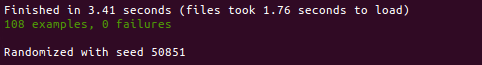
\includegraphics[scale=0.8]{images/rspec_result.png}
  \caption{Wyniki końcowe testów jednostkowych.}
  \label{fig:all_rspec}
\end{figure}

  \clearpage
  \subsection{Pokrycie kodu testami}
    Dzięki zstosowaniu technologi Ruby on Rails, mieliśmy do doyspozycji wiele ciekawych narzędzi pozwalających sprawdzać jakoś tworzonego kodu. Jednym z nich jest \emph{Stats}, który wykazuje pokrycie kodu testami.

    Statystyk wyliczana jest na podstawie ilości lini kodu (LOC - lines of code) do ilości lini testów (LOT - lines of test). Oczekiwanym wynikiem powinien być stosunek 1:2, który udało nam się osiągnąć.
    \begin{figure}[h]
      \centering
      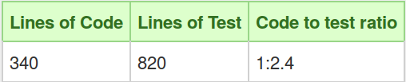
\includegraphics[scale=0.5]{images/loc_table.png}
      \caption{Statystyka pokrycia kodu testami}
    \end{figure}

    Poniżej załączyliśmy diagram obrazujący pokrycie kodu testami w okresie od 10 paździenika do 17 grudnia. Zanotowany duży skok, ilości lini kodu w stosunku do testów, był spowodowany złym zainkludowaniem bilbioteki javascript, która nie powinna być wliczana w metrykę.
    \begin{figure}[h]
      \centering
      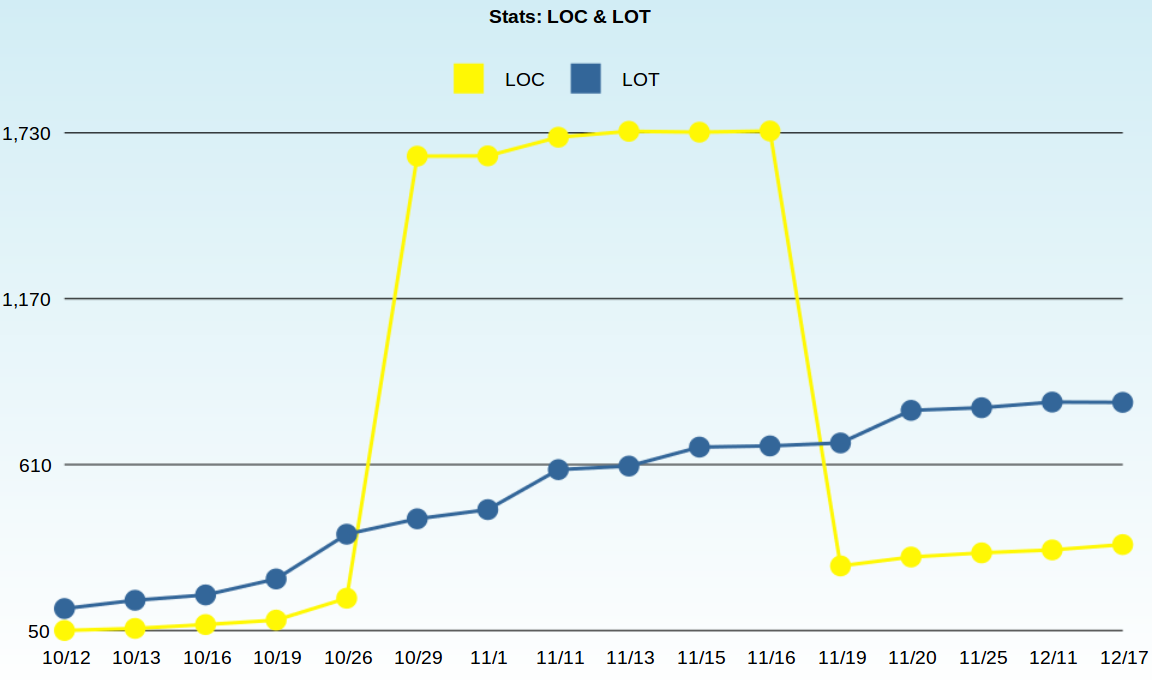
\includegraphics[scale=0.4]{images/LOC.png}
      \caption{Diagram pokrycia kodu testami [12.10-17.12]}
    \end{figure}
